\subsection*{Question 1}
	Soit on sait que $\dfrac{1}{5}=0,2$ et on multiplie par 2, soit on transforme la fraction pour pouvoir calculer le quotient $\dfrac{2}{5}=\dfrac{4}{10}=0,4$.

	C'est la réponse \textbf{C}.

\subsection*{Question 2}
	$30\,\%$ de 150 veut dire :\quad $150 \times \dfrac{30}{100}= 150 \times \dfrac{3}{10}= \dfrac{150}{10} \times 3= 15 \times 3=45$.

	C'est la réponse \textbf{C}.

\subsection*{Question 3}

\begin{minipage}{0.55\linewidth}
	Par lecture graphique, on observe que 1 est un antécédent de 3.

	C'est la réponse \textbf{B}.
\end{minipage}
	\hfill
	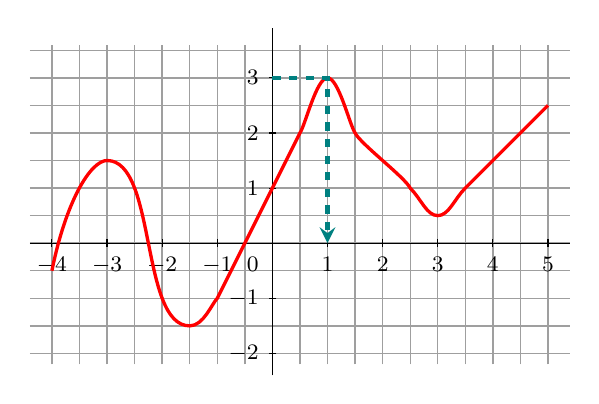
\begin{tikzpicture}[baseline={(current bounding box.center)},scale=0.7,>=stealth]
		\draw [color = gray!75, line width = 0.5pt, xstep=0.5, ystep = 0.5] (-4.4,-2.2) grid (5.4,3.6);
		\draw (-4.4,0) -- (5.4,0);
		\foreach \x in {-4,...,-1,1,2,...,5}
		\draw[shift={(\x,0)},color=black] (0pt,2pt) -- (0pt,-2pt) node[below] {\footnotesize $\np{\x}$};
		\draw (0,-2.4) -- (0,3.9);
		\foreach \y in {-2,-1,1,2,3}
		\draw[shift={(0,\y)},color=black] (2pt,0pt) -- (-2pt,0pt) node[left] {\footnotesize $\np{\y}$};
		\draw[color=black] (-2pt,-2pt) node[below left] {\footnotesize 0};
		\draw[line width=1.2pt,red]
		(-4,-0.5) .. controls (-3.75,0.75) and (-3.3,1.5) ..
		(-3,1.5) .. controls (-2.1 ,1.5 ) and (-2.4,-1.5) ..
		(-1.5,-1.5) .. controls (-1.25,-1.5 ) and (-1.1,-1.1) ..(-1,-1) --
		(0.5,2) .. controls (0.6,2.15 ) and (0.8,3) ..
		(1,3) .. controls (1.2,3) and (1.4,2.15 ) ..
		(1.5,2) .. controls (1.6,1.8) and (2.4,1.2) ..
		(2.5,1) .. controls (2.7,.8) and (2.8,0.5) ..
		(3,0.5) .. controls (3.2,0.5) and (3.3,0.8) ..
		(3.5,1) -- (5,2.5);
		\draw[teal, line width=1.5pt,dashed,->] (0,3)--(1,3)--(1,0);
	\end{tikzpicture}


\subsection*{Question 4}
	On résout l'équation $\begin{aligned}[t] 7 x+4 & = 5 x+ 6 \\
	7x-5x &= 6-4\\
	2x &= 2\\
	x &= 1
	\end{aligned}$

	L'équation a une solution : $x = 1$.

	C'est la réponse \textbf{D}.

\needspace{5\baselineskip}
\subsection*{Question 5}
	Le prix est d'abord multiplié par 0,9 puis par 1,1.

	$50 \times 0,9 \times 1,1= 5 \times 9 \times 1,1 = 45 \times 1,1 = 49,50$.

	\emph{Ou bien} : $0,9\times 1,1= 0,99$. \quad L'évolution globale est donc une baisse de 1\,\%, et 1\,\% de 50\,\euro{} c'est 0,50\,\euro{}.

	$50 - 0,5 = 49,5$.

	C'est la réponse \textbf{A}.

\subsection*{Question 6}
	Le point de la courbe d'abscisse $-1$ a pour ordonnée l'image de $-1$ par la fonction $x \mapsto 2 x^{2}-x+3$.

	$2 (-1)^{2}-(-1)+3=2+1+3=6$.

	L'image de $-1$ est 6, donc la courbe passe par le point de coordonnées $(-1 ; 6)$.

	C'est la réponse \textbf{D}.

\subsection*{Question 7}
	Le coefficient directeur de la droite (AB) est \quad $m=\dfrac{y_{\mathrm{B}}-y_{\mathrm{A}}}{x_{\mathrm{B}}-x_{\mathrm{A}}}=\dfrac{4-2}{-3-(-1)}=-1$.

	C'est la réponse \textbf{B}.

\subsection*{Question 8}
	Si on range les valeurs de la série dans l'ordre croissant, on obtient \quad $2 ; 2 ; 3 ; 3 ; 4 ; 5$.

	La série est composée d'un nombre pair de notes, donc la médiane est la moyenne des deux valeurs centrales, c'est-à-dire ici de la moyenne entre la 3\up{e} et la 4\up{e} valeur. Ces deux valeurs sont des 3, donc la médiane est 3.

	C'est la réponse \textbf{B}.


\needspace{10\baselineskip}
